\documentclass{article} % Especially this!

\usepackage[english]{babel}
\usepackage[utf8]{inputenc}
\usepackage[margin=1.5in]{geometry}
\usepackage{amsmath}
\usepackage{amsthm}
\usepackage{amsfonts}
\usepackage{amssymb}
\usepackage{graphicx}
\usepackage[siunitx]{circuitikz}
\usepackage{tikz}
\usepackage[colorinlistoftodos, color=orange!50]{todonotes}
\usepackage{hyperref}
\usepackage[numbers, square]{natbib}
\usepackage{fancybox}
\usepackage{epsfig}
\usepackage{soul}
\usepackage[framemethod=tikz]{mdframed}
\usepackage[shortlabels]{enumitem}
\usepackage[version=4]{mhchem}
\usepackage{multicol}
\usepackage{graphicx}
\graphicspath{ {./} }

\newcommand{\blah}{blah blah blah \dots}

\setlength{\marginparwidth}{3.4cm}

\newcommand{\summary}[1]{
\begin{mdframed}[nobreak=true]
\begin{minipage}{\textwidth}
\vspace{0.5cm}
\end{minipage}
\end{mdframed}}

\renewcommand*{\thefootnote}{\fnsymbol{footnote}}

\title{
\normalfont \large
\textsc{ASSIGNMENT-2
\vspace{10pt}
\\COL 216, Spring 2021} \\
[10pt] 
\rule{\linewidth}{0.5pt} \\[6pt] 
\Large Post-fix Expression Evaluation Using MIPS \\
\rule{\linewidth}{2pt}  \\[10pt]
}
\author{Jitender Kumar Yadav, 2019CS10361
\\Asha Ram Meena, 2019CS10337}
\date{\normalsize March 2, 2021}
\begin{document}

\maketitle
\section{Problem Statement}
\textbf{Write a MIPS Assembly Program for evaluating an expression in post-fix format.}

\section{Algorithm and Approach}
In a post-fix form of a numerical expression, all the numbers are on the left and the operators on the right. The evaluation starts at the middle and each operator takes two numbers just on the left and the evaluated value replaces the numbers and the operator. This yields another post-fix expression and this continues till a single number is left. The same algorithm can be achieved by use of stacks. In our example using MIPS, the post-fix expression is a string and the operands are simply digits.
\\The evaluation of post-fix expression is a standard algorithm and the following steps are used to evaluate the post-fix expression:
\begin{itemize}
    \item[$\diamond$] The string input on the console is read and stored in a variable.
    \item[$\diamond$] Each character is read, converted to the integer (digit) and pushed in the stack.
    \item[$\diamond$] In case there is any non-digit, an error is raised.
    \item[$\diamond$] The operators '+', '*' and '-' are checked one by one, the top two elements of the stack popped and the output of the operation is pushed back into the stack.
    \item[$\diamond$] If some other symbol apart from the operators appears, an error is raised.
    \item[$\diamond$] If the number of operators is less or more than the number corresponding to the operands available, an error is raised.
    \item[$\diamond$] In case the input is appropriate, the last element of the stack is popped and printed as output.
\end{itemize}

\section{Input and Output}
The input is to be taken from the user using console and the output shall be printed on the console itself. Suitable prompts shall be provided for the user for effective communication between the system and the user.
\subsection{Input Specifications:}
\begin{itemize}
    \item The input is a single line containing the post-fix expression without white spaces. Only allowed operators are +, - and *. The digits (from 0-9) of the strings are the operands.
\end{itemize}
\subsection{Output}
\begin{itemize}
    \item The output is a single integer, which is the evaluated value of the expression and is calculated and printed at the end.
\end{itemize}
\subsection{Sample I/O}
    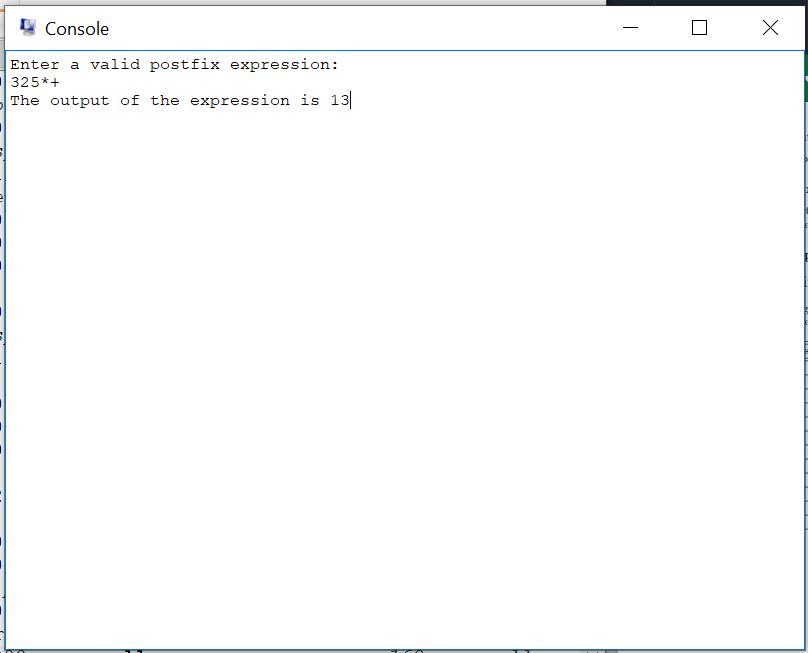
\includegraphics{sampleio_A2.JPG}

\section{Testing}
A variety of test cases were manually generated and evaluated to test the program. The test cases cover a vast majority of corner cases including single digit, no digit and invalid inputs.
\begin{table}[h]
    \centering
        \begin{tabular}{ |c|c|c|c| }
        \hline \hline
        Test Case & In-fix Expression & Prefix Expression & Expected Output \\
        \hline \hline
        1 & $3+2*5$ & $325*+$ & 13 \\
        \hline
        2 & $3$ & $3$ & 3 \\
        \hline
        3 & $4+1$ & $41+$ & 5 \\
        \hline
        4 & $3*2$ & $32*$ & 6 \\
        \hline
        5 & $7-2$ & $72-$ & 5 \\
        \hline
        6 & $3+7*(6-4)$ & 3764-*+ & 17 \\
        \hline
        7 & $4*(3-7)$ & $437-*$ & -16 \\
        \hline
        8 & $4-2*(1+1)$ & $4211+*-$ & 0 \\
        \hline
        9 & $-$ & $4211-+$ & Invalid Input \\
        \hline
        10 & $-$ & $4211-*++$ & Invalid Input \\
        \hline
        11 & $-$ & $-+$ & Invalid Input \\
        \hline
        12 & $-$ & $4211$ & Invalid Input \\
        \hline
        13 & $1*(2*(3*(4*(5*6))))$ & $123456*****$ & 720\\
        \hline
        14 & $2+(4*(5+(3*(3+4))))$ & $245334+*+*+$ & 106\\
        \hline
        15 & $9-(3+(1*(7-2)))$ & $93172-*+-$ & 1\\
        \hline
    \end{tabular}
    \caption{Test Cases}
    \label{tab:test_cases}
\end{table}
\end{document}